% ---------------------------------- DESIGN -------------------------------------

\chapter{Design}

\begin{comment}
In questo capitolo si spiegano le strategie messe in campo per realizzare la soluzione ai problemi identificati nell'analisi.

Si parte da una visione architetturale, il cui scopo è informare il lettore di quale sia il funzionamento dell'applicativo realizzato ad alto livello.
%
In particolare, è necessario descrivere accuratamente in che modo i componenti principali del sistema si coordinano fra loro.
%
A seguire, si dettagliano alcune parti del design, quelle maggiormente rilevanti al fine di chiarificare la logica con cui sono stati risolti i problemi dell'applicazione.
\end{comment}

\section{Architettura}

\textsf{\small L'obiettivo del team era quello di poter lavorare ognuno alla propria parte indipendentemente ed evitando conflitti, per poi poterle collegare tutte assieme alla fine.}\\

\textsf{\small Il progetto sfrutta quindi il pattern architetturale \textbf{MVC} (\emph{M}odel \emph{V}iew \emph{C}ontroller) che permette di suddividere la gestione dell'applicativo in tre parti separate: }\\

\begin{itemize} %TODO: ingrandire questa parte oppure scrivere di più nell'introduzione del Design.
	\item \textsf{\small \textbf{Model}: dove vengono effettivamente modellate le entità di gioco. In questa parte vengono gestiti tutti gli aspetti riguardanti la logica, la gestione, la fisica, le caratteristiche e il comportamento delle componenti di gioco.}
	%si occupa dell'interfaccia grafica
	\item \textsf{\small \textbf{View}: si occupa degli aspetti grafici, quali esporre le effettive entità del \emph{Model} sullo schermo di gioco. La \emph{View} comprende anche il menù di gioco e la schermata di fine partita per esaminare i risultati della classifica. Riguarda, inoltre, anche la parte di generazione delle mappa che comprende vari tipi di sfondi e relative piattaforme in tema, monete, oggetti, armi e nemici.}
	% Inoltre, riguarda anche
	\item \textsf{\small \textbf{Controller}: è il concreto ponte, tra il \emph{Model} e la \emph{View}, consente di collegare la parte logica con quella visiva. La sua funzione è quella di ricevere input della tastiera dall'utente, inviarlo al \emph{Model} per essere elaborato e alla \emph{View} per avere un riscontro visivo.}
\end{itemize}

\textsf{\small Di seguito, un UML riguardante il pattern architetturale \textbf{MVC} utilizzato:}\\

\begin{figure}[htp]
	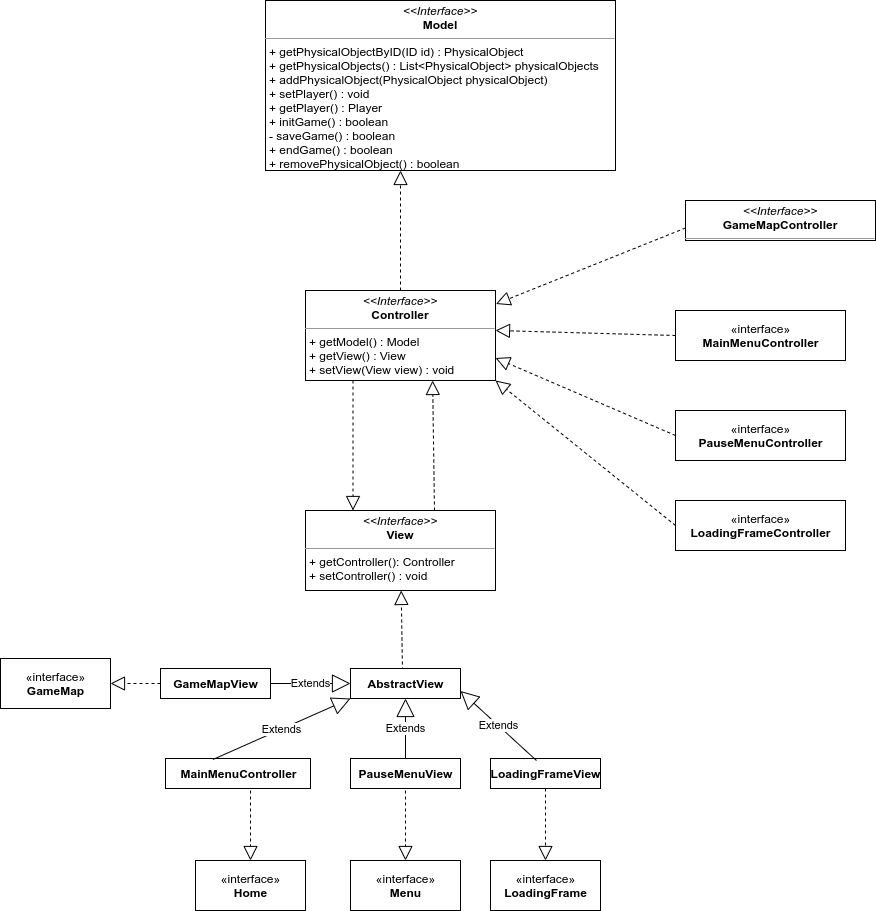
\includegraphics[width=1.2\linewidth]{./img/mvc.png}
	\caption{Schema UML del pattern architetturale MVC.}
	\label{img:mvc}
\end{figure}

%\newpage

\begin{comment}

Questa sezione spiega come le componenti principali del software interagiscono fra loro.
%
In particolare, qui va spiegato \textbf{se} e \textbf{come} è stato utilizzato il pattern
architetturale model-view-controller (e/o alcune sue declinazioni specifiche, come entity-control-boundary).

Se non è stato utilizzato MVC, va spiegata in maniera molto accurata l'architettura scelta, giustificandola in modo appropriato.

Se è stato scelto MVC, vanno identificate con precisione le interfacce e classi che rappresentano i punti d'ingresso per modello, view, e controller.
Raccomandiamo di sfruttare la definizione del dominio fatta in fase di analisi per capire quale sia l'entry point del model, e di non realizzare un'unica macro-interfaccia che, spesso, finisce con l'essere il prodromo ad una ``God class''.
%
Consigliamo anche di separare bene controller e model, facendo attenzione a non includere nel secondo strategie d'uso che appartengono al primo.

In questa sezione vanno descritte, per ciascun componente architetturale che ruoli ricopre (due o tre ruoli al massimo), ed in che modo interagisce (ossia, scambia informazioni) con gli altri componenti dell'architettura.
%
Raccomandiamo di porre particolare attenzione al design dell'interazione fra view e controller: se ben progettato, sostituire in blocco la view non dovrebbe causare alcuna modifica nel controller (tantomeno nel model).

\subsection*{Elementi positivi}
\begin{itemize}
	\item Si mostrano pochi, mirati schemi UML dai quali si deduce con chiarezza quali sono le parti principali del software e come interagiscono fra loro.
	\item Si mette in evidenza se e come il pattern architetturale model-view-controller è stato applicato, anche con l'uso di un UML che mostri le interfacce principali ed i rapporti fra loro.
	\item Si discute se sia semplice o meno, con l'architettura scelta, sostituire in blocco la view: in un MVC ben fatto, controller e modello non dovrebbero in alcun modo cambiare se si transitasse da una libreria grafica ad un'altra (ad esempio, da Swing a JavaFX, o viceversa).
\end{itemize}

\subsection*{Elementi negativi}
\begin{itemize}
	\item L'architettura è fatta in modo che sia impossibile riusare il modello per un software diverso che affronta lo stesso problema.
	\item L'architettura è tale che l'aggiunta di una funzionalità sul controller impatta pesantemente su view e/o modello.
	\item L'architettura è tale che la sostituzione in blocco della view impatta sul controller o, peggio ancora, sul modello.
	\item Si presentano UML caotici, difficili da leggere.
	\item Si presentano UML in cui sono mostrati elementi di dettaglio non appartenenti all'architettura, ad esempio includenti campi o con metodi che non interessano la parte di interazione fra le componenti principali del software.
	\item Si presentano schemi UML con classi (nel senso UML del termine) che ``galleggiano'' nello schema, non connesse, ossia senza relazioni con il resto degli elementi inseriti.
	\item Si presentano elementi di design di dettaglio, ad esempio tutte le classi e interfacce del modello o della view.
	\item Si discutono aspetti implementativi, ad esempio eventuali librerie usate oppure dettagli di codice.
\end{itemize}

\subsection*{Esempio}

L'architettura di GLaDOS segue il pattern architetturale MVC.
%
Più nello specifico, a livello architetturale, si è scelto di utilizzare MVC in forma ``ECB'', ossia ``entity-control-boundary''\footnote{
	Si fa presente che il pattern ECB effettivamente esiste in letteratura come ``istanza'' di MVC, e chi volesse può utilizzarlo come reificazione di MVC.
}.
%
GLaDOS implementa l'interfaccia AI, ed è il controller del sistema.
Essendo una intelligenza artificiale, è una classe attiva.
%
GLaDOS accetta la registrazione di Input ed Output, che fanno parte della ``view'' di MVC, e sono il ``boundary'' di ECB.
Gli Input rappresentano delle nuove informazioni che vengono fornite all'IA, ad esempio delle modifiche nel valore di un sensore, oppure un comando da parte dell'operatore.
Questi input infatti forniscono eventi.
Ottenere un evento è un'operazione bloccante: chi la esegue resta in attesa di un effettivo evento.
Di fatto, quindi, GLaDOS si configura come entità \textit{reattiva}.
Ogni volta che c'è un cambio alla situazione del soggetto, GLaDOS notifica i suoi Output,
informandoli su quale sia la situazione corrente.
%
Conseguentemente, GLaDOS è un ``observable'' per Output.

\begin{figure}[h]
	\centering{}
	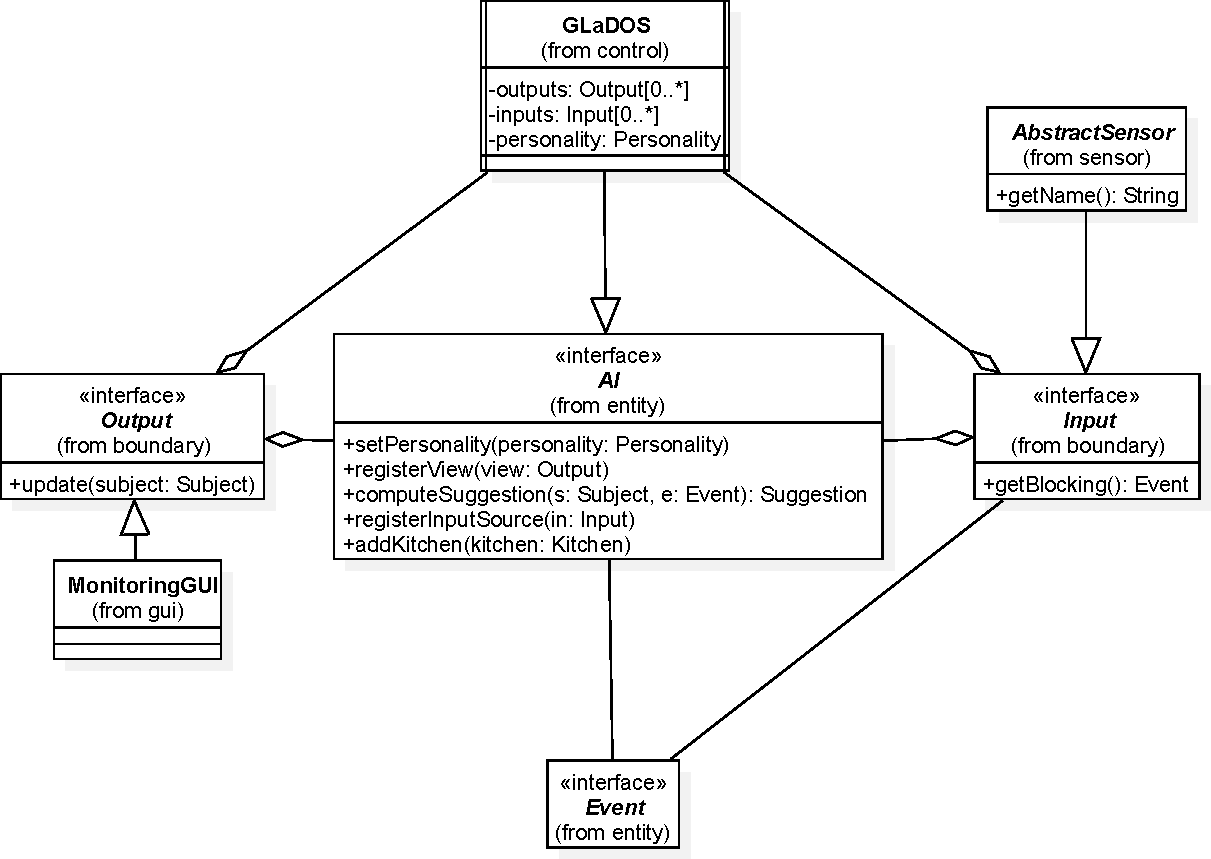
\includegraphics[width=\textwidth]{img/arch}
	\caption{Schema UML architetturale di GLaDOS. L'interfaccia \texttt{GLaDOS} è il controller del sistema, mentre \texttt{Input} ed \texttt{Output} sono le interfacce che mappano la view (o, più correttamente in questo specifico esempio, il boundary). Un'eventuale interfaccia grafica interattiva dovrà implementarle entrambe.}
	\label{img:goodarch}
\end{figure}

Con questa architettura, possono essere aggiunti un numero arbitrario di input ed output
all'intelligenza artificiale.
%
Ovviamente, mentre l'aggiunta di output è semplice e non richiede alcuna modifica all'IA, la
presenza di nuovi tipi di evento richiede invece in potenza aggiunte o rifiniture a GLaDOS.
%
Questo è dovuto al fatto che nuovi Input rappresentano di fatto nuovi elementi della business
logic, la cui alterazione od espansione inevitabilmente impatta il controller del progetto.

In \Cref{img:goodarch} è esemplificato il diagramma UML architetturale.

\end{comment}

\section{Design dettagliato}

%TODO: commentare questa parte del prof. quando avremo tutti finito di scrivere la nostra. -----------------  INIZIO -----------------------------------

In questa sezione si possono approfondire alcuni elementi del design con maggior dettaglio.
%
Mentre ci attendiamo principalmente (o solo) interfacce negli schemi UML delle sezioni precedenti, in questa sezione è necessario scendere in maggior dettaglio presentando la struttura di alcune sottoparti rilevanti dell'applicazione.
%
È molto importante che, descrivendo un problema, quando possibile si mostri che non si è re-inventata la ruota ma si è applicato un design pattern noto.
%
È assolutamente inutile, ed è anzi controproducente, descrivere classe-per-classe (o peggio ancora metodo-per-metodo) com'è fatto il vostro software: è un livello di dettaglio proprio della documentazione dell'API (deducibile dalla Javadoc).

\textbf{È necessario che ciascun membro del gruppo abbia una propria sezione di design dettagliato,
	di cui sarà il solo responsabile}.
%
Ciascun autore dovrà spiegare in modo corretto e giustamente approfondito (non troppo in dettaglio, non superficialmente) il proprio contributo.
%
È importante focalizzarsi sulle scelte che hanno un impatto positivo sul riuso, sull'estensibilità, e sulla chiarezza dell'applicazione.
%
Esattamente come nessun ingegnere meccanico presenta un solo foglio con l'intero progetto di una vettura di Formula 1, ma molteplici fogli di progetto che mostrano a livelli di dettaglio differenti le varie parti della vettura e le modalità di connessione fra le parti, così ci aspettiamo che voi, futuri ingegneri informatici, ci presentiate prima una visione globale del progetto, e via via siate in grado di dettagliare le singole parti, scartando i componenti che non interessano quella in esame.
%
Per continuare il parallelo con la vettura di Formula 1, se nei fogli di progetto che mostrano il
design delle sospensioni anteriori appaiono pezzi che appartengono al volante o al turbo, c'è una
chiara indicazione di qualche problema di design.

Usare correttamente i design pattern in questa sezione è molto importante: se vengono utilizzati correttamente, è molto probabile riuscire a progettare il software in modo corretto, estensibile, e riusabile.
%
Per ogni pattern utilizzato si presenti:
\begin{itemize}
	\item almeno un paragrafo che spieghi come è reificato nel progetto (ad esempio: nel caso di Template Method, qual è il metodo template; nel caso di Strategy, quale interfaccia del progetto rappresenta la strategia, e quali sono le sue implementazioni; nel caso di Decorator, qual è la classe astratta che fa da Decorator e quali sono le sue implementazioni concrete; eccetera);
	\item almeno uno schema UML che grafichi quanto sopra descritto.
\end{itemize}
%
La presenza di pattern di progettazione \emph{correttamente utilizzati} è valutata molto positivamente.
%
L'uso inappropriato è invece valutato negativamente: a tal proposito, si raccomanda di porre particolare attenzione all'abuso di Singleton, che, se usato in modo inappropriato, è di fatto un anti-pattern.

\subsection*{Elementi positivi}

\begin{itemize}
	\item Ogni membro del gruppo discute le proprie decisioni di progettazione, ed in particolare le azioni volte ad anticipare possibili cambiamenti futuri (ad esempio l'aggiunta di una nuova funzionalità, o il miglioramento di una esistente).
	\item Si identificano, utilizzano \textit{appropriatamente}, e descrivono come suggerito diversi design pattern.
	\item Ogni membro del gruppo identifica i pattern utilizzati nella sua sottoparte.
	\item Si mostrano gli aspetti di design più rilevanti dell'applicazione, mettendo in luce la maniera in cui si è costruita la soluzione ai problemi descritti nell'analisi.
	\item Si tralasciano aspetti strettamente implementativi e quelli non rilevanti, non mostrandoli negli schemi UML (ad esempio, campi privati) e non descrivendoli.
	\item Si mostrano le principali interazioni fra le varie componenti che collaborano alla soluzione di un determinato problema.
	\item Ciascun design pattern identificato presenta una piccola descrizione del problema calato
	nell'applicazione, uno schema UML che ne mostra la concretizzazione nelle classi del progetto, ed
	una breve descrizione della motivazione per cui tale pattern è stato scelto. Ad esempio, se si
	dichiara di aver usato Observer, è necessario specificare chi sia l'observable e chi l'observer; se
	si usa Template Method, è necessario indicare quale sia il metodo template; se si usa Strategy, è
	necessario identificare l'interfaccia che rappresenta la strategia; e via dicendo.
\end{itemize}

\subsection*{Elementi negativi}
\begin{itemize}
	\item Il design del modello risulta scorrelato dal problema descritto in analisi.
	\item Si tratta in modo prolisso, classe per classe, il software realizzato.
	\item Non si presentano schemi UML esemplificativi.
	\item Non si individuano design pattern, o si individuano in modo errato (si spaccia per design pattern qualcosa che non lo è).
	\item Si utilizzano design pattern in modo inopportuno. Un esempio classico è l'abuso di
	Singleton per entità che possono essere univoche ma non devono necessariamente esserlo. Si rammenta
	che Singleton ha senso nel secondo caso (ad esempio \texttt{System} e \texttt{Runtime} sono
	singleton), mentre rischia di essere un problema nel secondo. Ad esempio, se si rendesse singleton
	il motore di un videogioco, sarebbe impossibile riusarlo per costruire un server per partite online
	(dove, presumibilmente, si gestiscono parallelamente più partite).
	\item Si producono schemi UML caotici e difficili da leggere, che comprendono inutili elementi
	di dettaglio.
	\item Si presentano schemi UML con classi (nel senso UML del termine) che ``galleggiano'' nello schema, non connesse, ossia senza relazioni con il resto degli elementi inseriti.
	\item Si tratta in modo inutilmente prolisso la divisione in package, elencando ad esempio le classi una per una.
\end{itemize}

\subsection*{Esempio minimale (e quindi parziale) di sezione di progetto con UML ben realizzati}

In questa sezione ci si concentrerà sugli aspetti di personalità e sul funzionamento del reporting di GLaDOS.

Il sistema per la gestione della personalità utilizza il pattern Strategy, come da
\Cref{img:strategy}: le implementazioni di \texttt{Personality} possono essere modificate, e la
modifica impatta direttamente sul comportamento di GLaDOS.

\begin{figure}[h]
	\centering{}
	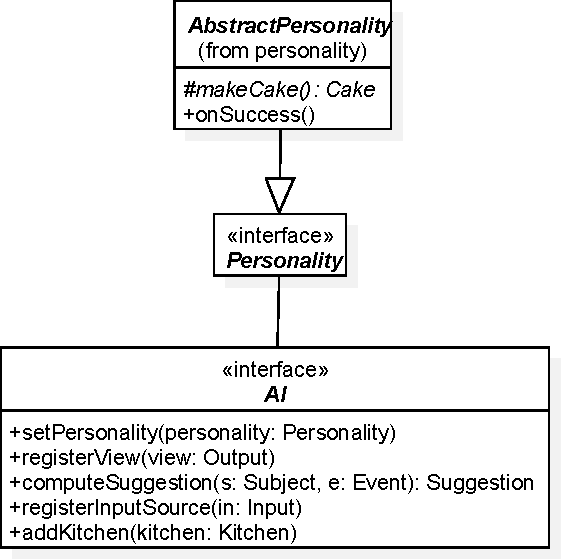
\includegraphics[width=\textwidth]{img/strategy}
	\caption{Rappresentazione UML del pattern Strategy per la personalità di GLaDOS}
	\label{img:strategy}
\end{figure}

\begin{figure}[h]
	\centering{}
	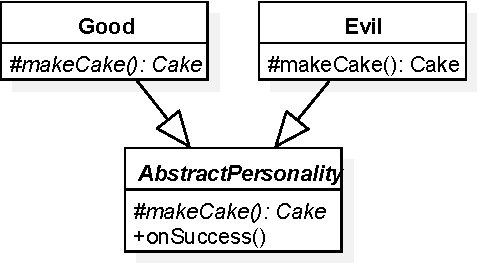
\includegraphics[width=\textwidth]{img/template}
	\caption{Rappresentazione UML dell'applicazione del pattern Template Method alla gerarchia delle Personalità}
	\label{img:template}
\end{figure}

Sono state attualmente implementate due personalità, una buona ed una cattiva.
Quella buona restituisce sempre una torta vera, mentre quella cattiva restituisce sempre la
promessa di una torta che verrà in realtà disattesa.
Dato che le due personalità differiscono solo per il comportamento da effettuarsi in caso di percorso completato con successo, è stato utilizzato il pattern template method per massimizzare il riuso, come da \Cref{img:template}.
Il metodo template è \texttt{onSuccess()}, che chiama un metodo astratto e protetto
\texttt{makeCake()}.

\begin{figure}[h]
	\centering{}
	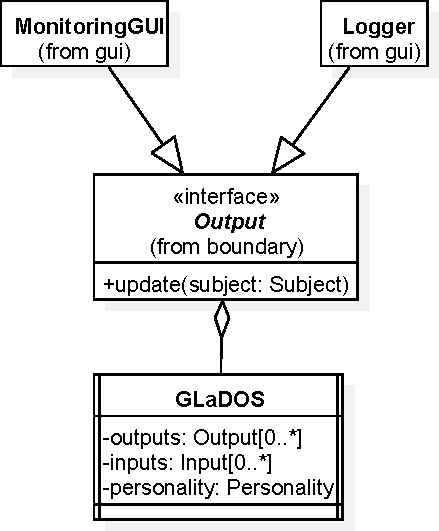
\includegraphics[width=.7\textwidth]{img/observer}
	\caption{Il pattern Observer è usato per consentire a GLaDOS di informare tutti i sistemi di output in ascolto}
	\label{img:observer}
\end{figure}

Per quanto riguarda il reporting, è stato utilizzato il pattern Observer per consentire la
comunicazione uno-a-molti fra \texttt{GLaDOS} ed i sistemi di output.
%
\texttt{GLaDOS} è observable, e le istanze di \texttt{Input} sono observer.
%
Il suo utilizzo è esemplificato in \Cref{img:observer}

\subsection*{Contro-esempio: pessimo diagramma UML}

In \Cref{img:badarch} è mostrato il modo \textbf{sbagliato} di fare le cose.
%
Questo schema è fatto male perché:
\begin{itemize}
	\item È caotico.
	\item È difficile da leggere e capire.
	\item Vi sono troppe classi, e non si capisce bene quali siano i rapporti che intercorrono fra loro.
	\item Si mostrano elementi implementativi irrilevanti, come i campi e i metodi privati nella classe \texttt{AbstractEnvironment}.
	\item Se l'intenzione era quella di costruire un diagramma architetturale, allora lo schema è ancora più sbagliato, perché mostra pezzi di implementazione.
	\item Una delle classi, in alto al centro, galleggia nello schema, non connessa a nessuna altra classe, e di fatto costituisce da sola un secondo schema UML scorrelato al resto
	\item Le interfacce presentano tutti i metodi e non una selezione che aiuti il lettore a capire quale parte del sistema si vuol mostrare.
\end{itemize}


\begin{figure}[h]
	\centering{}
	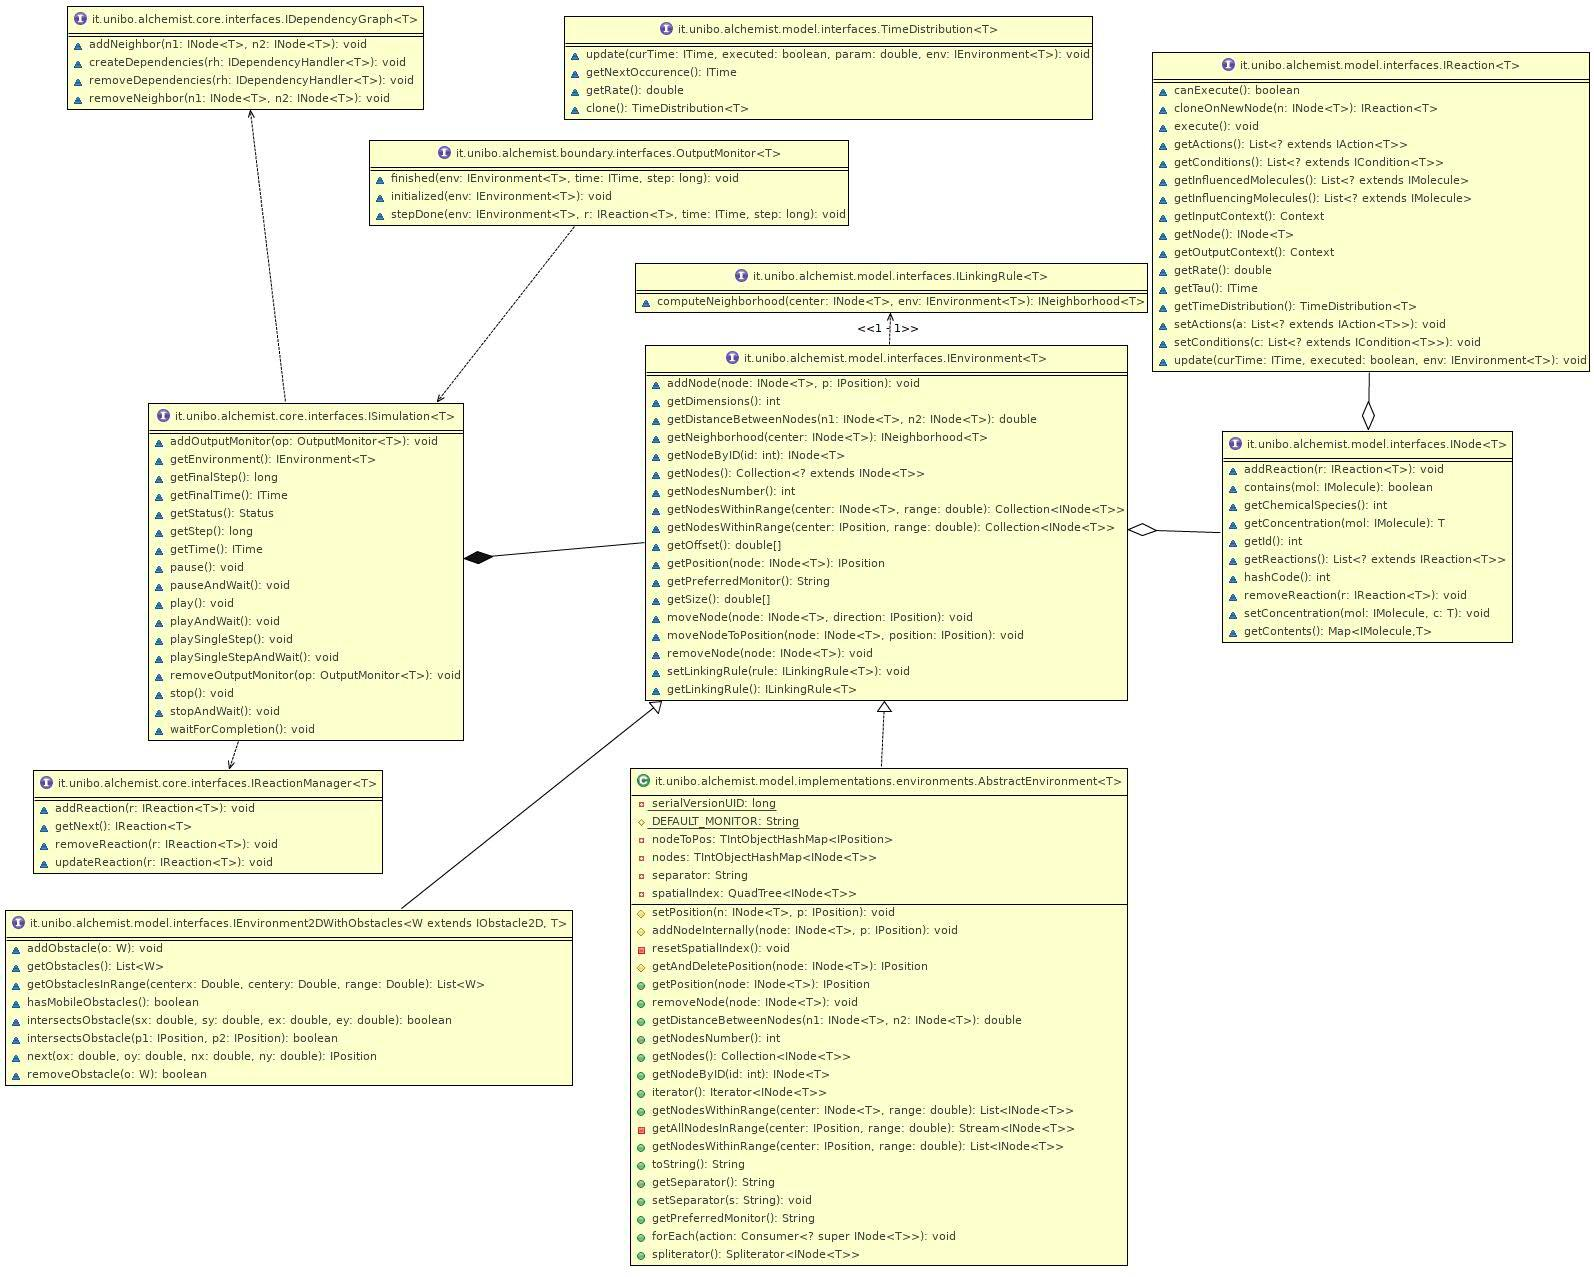
\includegraphics[width=\textwidth]{img/badarch}
	\caption{Schema UML mal fatto e con una pessima descrizione, che non aiuta a capire. Don't try this at home.}
	\label{img:badarch}
\end{figure}

%TODO: commentare questa parte del prof. quando avremo tutti finito di scrivere la nostra. -----------------  FINE -----------------------------------

% ----------------- ALESSANDRO PIOGGIA -----------------------------------------

\newpage

\subsection*{Alessandro Pioggia}
\textbf{Physical objects} \\ \\
Lo scopo iniziale del progetto è stato quello di creare delle vere e proprie entità di gioco(Players, Enemies, Obstacles, Items), che potessero popolare la mappa e interagire fra loro.
La mia parte richiedeva che io costruissi il core delle entità fisiche di gioco(oltre all'implementazione di alcune di esse), in modo da poter creare una struttura solida alla quale potessero fare riferimento i colleghi, sfruttando il principio della generalizzazione.
L'interfaccia PhysicalObject rappresenta la struttura base di una entità di gioco, la quale è composta da una dimensione, una posizione e contiene un riferimento all'ambiente di gioco. \\ \\

\begin{figure}[H]
	\centering{}
	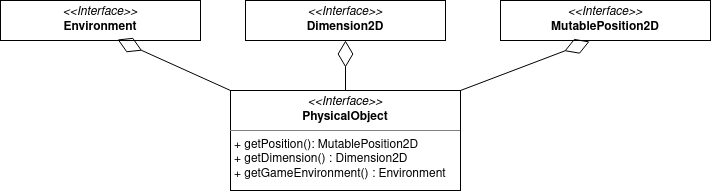
\includegraphics[width=\textwidth]{img/physicalObject}
	\label{img:physicalObject}
	\caption{Schema UML rappresentante l'interfaccia PhysicalObject con relative dipendenze. \\}
\end{figure}

\newpage

\textbf{AbstractStaticComponent e AbstractDynamicComponent} \\ \\
A livello implementativo è stato scelto di separare le entità di gioco statiche da quelle dinamiche.
Le entità statiche una volta istanziate non possono cambiare posizione, mentre quelle dinamiche possono muoversi in qualsiasi momento e sono dotate di una propria velocità. A questo proposito ho scelto di implementare le due componenti creando due classi astratte che implementassero l'interfaccia PhysicalObject, semplificando la creazione di classi di specializzazione.

\begin{figure}[H]
	\centering{}
	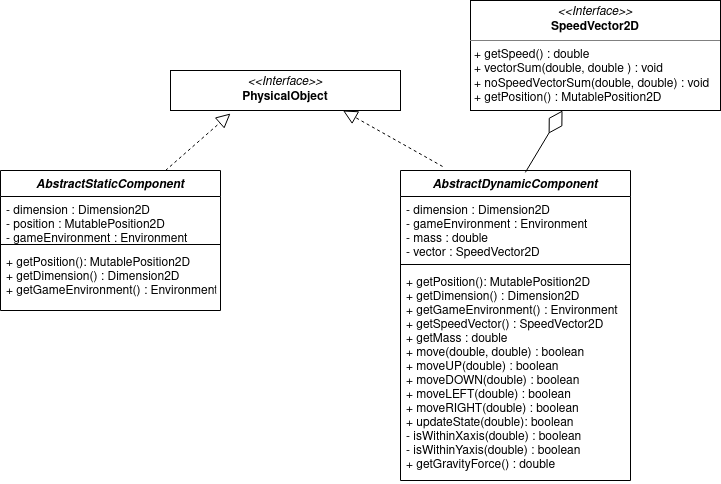
\includegraphics[width=\textwidth]{img/components}
	\label{img:components.png}
	\caption{Schema UML rappresentante le classi astratte riguardanti le entità fisiche statiche e dinamiche. \\}
\end{figure}

\newpage

\textbf{Item} \\ \\
Gli Item sono entità presenti all'interno dell'ambiente di gioco, i quali possono essere raccolti dal main player, il quale ne subisce l'effetto.
In questa situazione ho deciso di creare due DynamicPickupItem e StaticPickupItem che estendono rispettivamente AbstractDynamicComponent e AbstractStaticComponent.
Similmente ho creato gli staticObstacle e dynamicObstacle.
Per semplificare l'istanziamento ho deciso di utilizzare il factory pattern, il quale è tornato molto utile e ha ridotto la verbosità.

\begin{figure}[H]
	\centering{}
	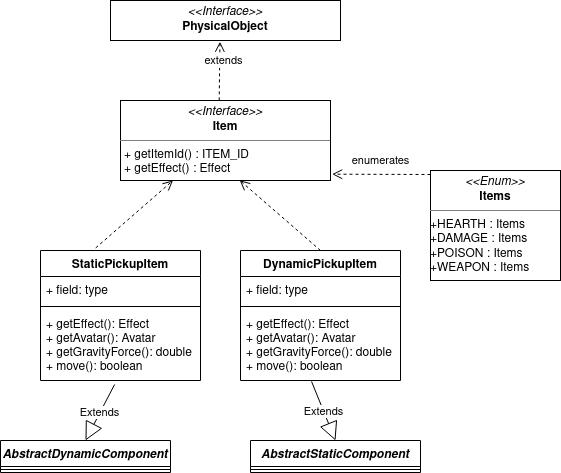
\includegraphics[width=\textwidth]{img/item}
	\label{img:item.png}
	\caption{Schema UML rappresentante gli Item di gioco\\}
\end{figure}

\begin{figure}[H]
	\centering{}
	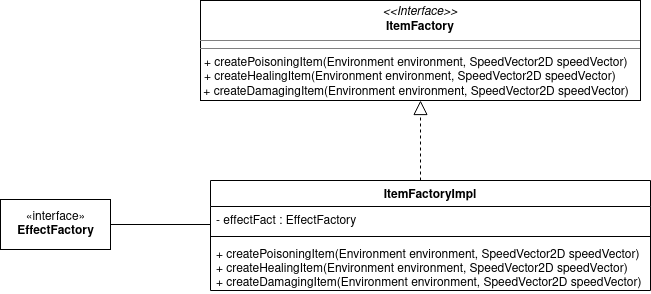
\includegraphics[width=\textwidth]{img/ItemFactory}
	\label{img:ItemFactory.png}
	\caption{Schema UML rappresentante il factory pattern applicato agli Item\\}
\end{figure}

\newpage

\textbf{Main menu} \\ \\

Il main menu non è altro che il menù principale, ovvero quello che viene visualizzato all'avvio dell'applicazione e permette all'utente di decidere se e quando iniziare a giocare.
Per realizzarlo ho deciso di sfruttare scene builder, software che mi ha permesso di generare i file fxml, ai quali sono stati associati dei controller, permettendomi di solidificare il concetto di separation of concerns. \\ \\

\begin{figure}[H]
	\centering{}
	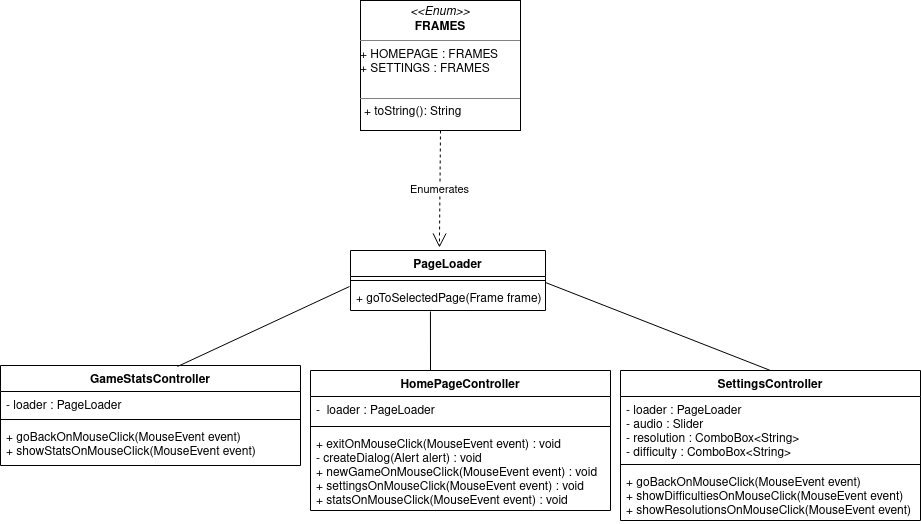
\includegraphics[width=\textwidth]{img/main_menu}
	\label{img:main_menu.png}
	\caption{Schema UML rappresentante il main menu\\}
\end{figure}


% ----------------- LEON BAIOCCHI -----------------------------------------

\newpage

\subsection*{Leon Baiocchi}

% ----------------- FEDERICO BRUNELLI -----------------------------------------

\newpage

\subsection*{Federico Brunelli}

% ----------------- LUCA RENGO -----------------------------------------

\newpage

\subsection*{Luca Rengo}

\textsf{\small La mia parte riguardava l'implementazione dei personaggi di gioco e dei diversi aspetti riguardanti la generazione della mappa e dei suoi componenti a livello di \emph{View}.}\\

\textsf{\small Mi competeva, inoltre, l'inizializzazione delle varie scene di gioco, dell'implementazione delle sprites, del salvataggio dei punteggi e delle statistiche completati dal giocatore.}\\ 
%della generazione della mappa a livello di \emph{View}.}\\

\subsubsection*{Characters}

\textsf{\small Per quanto concerne l'implementazione dei personaggi di gioco, ho sviluppato un'interfaccia \emph{Characters} che pone a tutte le figure l'implementazione di un contratto con le varie azioni comuni, i vari metodi che un personaggio può eseguire.}\\

\textsf{\small Questo è stato trattato dalle classi \emph{Player} ed \emph{Enemy} che contengono le proprietà e caratteristiche dei personaggi come la loro vita, il mana, il nome, le loro abilità e capacità come quella di muoversi e saltare.}\\

\textsf{\small Ho utilizzato poi un enum, \emph{EntityList}, per poter rappresentare diversi tipi di personaggi con diverse caratteristiche che ho settato nel metodo \emph{setPlayerType()} e \emph{setEnemyType()} delle rispettive classi. }\\

\textsf{\small Mi sono avvalso, inoltre, del pattern architetturale \textbf{Factory} per raccogliere le varie tipologie di \emph{Player} ed \emph{Enemy} attraverso l'interfaccia \emph{FactoryCharacters} e la sua implementazione \emph{FactoryCharactersImpl} per riorganizzare meglio i vari personaggi del gioco e rendere la loro creazione più chiara e semplice, evitando così di dover passare, ogni volta, un eccessivo numero di parametri da inizializzare.}

%TODO: immagine Model

\begin{figure}[h]
	\centering{} %TODO: aggiungere immagine UML
	%\includegraphics[width=\textwidth]{} 
	\caption{Schema UML del \emph{Model} relativo ai \emph{Characters}.}
	\label{img:uml_model_characters}
\end{figure}

\subsubsection*{Mappa di gioco} %TODO: approfondire la spiegazione. Descrivere le difficoltà incontrate e le soluzioni.

\textsf{\small Per quanto riguarda la \emph{Mappa} mi sono occupato degli aspetti della \emph{View}.}\\

\textsf{\small E' presente l'interfaccia \emph{GameView} che viene implementata dalla classe astratta \emph{AbstractScene} che ha il compito di rappresentare una generica scena del gioco, come la mappa o i crediti del gioco. Questa è ereditata dalla Classe \emph{MapScene} che implementa una specifica scena del gioco, ovvero quella della mappa, inizializzando tutte le sprites delle varie entità di gioco e generandole sullo schermo.}\\

\textsf{\small In \emph{MapScene} vengono generate le sprites dalle classi \emph{Platform}, \emph{Coin}, \emph{MainEnemy}, \emph{MainPlayer} con la sua animazione implementata in \emph{SpriteAnimation}.}\\

\textsf{\small Queste entità vengono posizionate in una precisa posizione in base alla locazione di un carattere in un array di stringhe che si trova nella classe \emph{LevelData}.} %TODO: sistemare, scrivere meglio.

\textsf{\small Ad ogni entità del gioco è associato un carattere che si trova nell'array di stringhe in \emph{LevelData}.}\\ %TODO: anche qui.

\textsf{\small Le classi \emph{Platform} e \emph{Coin} sono simili ed entrambe hanno un proprio enum per le proprie varie tipologie e utilizzano una ImageView per settare l'immagine, le proprietà e le posizioni sullo schermo.}\\

\textsf{\small \emph{MainEnemy} è una semplice ImageView statica mentre \emph{MainPlayer} è una ImageView dinamica, ovvero con un'animazione.}
\textsf{\small \emph{SpriteAnimation} è la classe che carica da \emph{MainPlayer} l'immagine e le sue caratteristiche (come width dell'immagine, height, ecc..) ed interpola le varie immagini della spritesheet del giocatore per creare la sua animazione che dura tot millisecondi.}\\

\textsf{\small  Quale sfondo della mappa da mostrare e la relativa piattaforma in tema e quale moneta vengono settate nella classe \emph{Map} che tiene traccia di questi elementi della View.}\\

%TODO: inserire UML della parte della mappa di gioco.

%TODO: parlare della Mappa (Map, MapScene, AbstractScene), del MainPlayer, SpriteAnimation, MainEnemy, Platform, Coin. LevelData

\subsubsection*{Salvataggio}

\textsf{\small Per quanto riguarda l'operazione di salvataggio delle statistiche di gioco, mi sono avvalso della classe \emph{Save} che crea un file di salvataggio in cui vengono contenuti il nome dei giocatori e i loro relativi punteggi.}\\

\textsf{\small Per fare questo, usufruisco di un \emph{BufferedWriter} per creare il file qualora questo non esista già. Altrimenti, mi limito ad aggiungere i dati in coda al file per evitare di eliminare ciò che era stato precedentemente memorizzato.}\\

\textsf{\small Poi mi avvalgo di un \emph{BufferedReader} per leggere dal file e memorizzare i dati e restituire un \emph{HashMap<String, Integer>} con il nome del player e il suo relativo punteggio.}\\

\textsf{\small Infine, ho un metodo per resettare il file e cancellare tutti i dati che erano stati immagazzinati.}\\

%TODO: aggiungere UML del salvataggio.